% UG project example file, February 2022
% Do not change the first two lines of code, except you may delete "logo," if causing problems.
% Understand any problems and seek approval before assuming it's ok to remove ugcheck.
\documentclass[logo,bsc,singlespacing,parskip]{infthesis}
\usepackage{ugcheck}
\usepackage{multicol}
\usepackage{dirtree}
\usepackage{graphicx} 

% Include any packages you need below, but don't include any that change the page
% layout or style of the dissertation. By including the ugcheck package above,
% you should catch most accidental changes of page layout though.

\usepackage{microtype} % recommended, but you can remove if it causes problems
%\usepackage{natbib}
\usepackage[hidelinks]{hyperref}
\usepackage{csquotes}

\begin{document}
\begin{preliminary}

\title{Concurrent Web Development with Effect Handlers in Links}

\author{Steven Chang}

% CHOOSE YOUR DEGREE a):
% please leave just one of the following un-commented
\course{Electronics and Computer Science}
%\course{Artificial Intelligence and Computer Science}
%\course{Artificial Intelligence and Mathematics}
%\course{Artificial Intelligence and Software Engineering}
%\course{Cognitive Science}
%\course{Computer Science}
%\course{Computer Science and Management Science}
%\course{Computer Science and Mathematics}
%\course{Computer Science and Physics}
%\course{Software Engineering}
%\course{Master of Informatics} % MInf students

% CHOOSE YOUR DEGREE b):
% please leave just one of the following un-commented
%\project{MInf Project (Part 1) Report}  % 4th year MInf students
%\project{MInf Project (Part 2) Report}  % 5th year MInf students
\project{4th Year Project Report}        % all other UG4 students


\date{\today}

\abstract{
TODO
}

\maketitle

\newenvironment{ethics}
   {\begin{frontenv}{Research Ethics Approval}{\LARGE}}
   {\end{frontenv}\newpage}

\begin{ethics}
% IF ETHICS APPROVAL WAS NOT REQUIRED:
This project was planned in accordance with the Informatics Research
Ethics policy. It did not involve any aspects that required approval
from the Informatics Research Ethics committee.

\standarddeclaration
\end{ethics}


\begin{acknowledgements}

\end{acknowledgements}


\tableofcontents
\end{preliminary}


\chapter{Introduction}

TODO: This paragraph might be better for abstract

This report explores the use of effect handlers in web development using the Links programming language. The primary objective is to enhance the user-friendliness and accessibility of concurrent programming with effect handlers by allowing users to easily define and switch their own handlers within the client code. The project achieves this by implementing various web applications and user-level thread schedulers using Links and effect handlers, with a focus on enabling users to switch between different effect handlers with minimal changes to the client code. The project successfully demonstrates a proof of concept that encapsulates effect handlers as independent modules, offering a more efficient and flexible approach for concurrent programming in the context of web development using effect handlers.

\section{Motivations}

Links \cite{links_website} is a functional programming language that aims to simplify web programming by providing a unified language for all tiers of a web application, which includes the client-side, server-side, and database. To achieve this, Links translates code into the appropriate languages for each tier, such as JavaScript for the browser, Java for the server, and SQL for the database. Additionally, Links supports features that facilitate web development, including manipulation of the Document Object Model (DOM) and event listeners \cite{links}. Furthermore, Links allows for concurrency on both the client and server-side \cite{links}, which enables users to create web applications that can handle multiple tasks simultaneously.

In contrast to conventional web development technologies, Links offers effect handlers \cite{daniel_effect_links} as an abstraction for managing effects such as exceptions, input/output operations, and state changes in a modular and composable way. An effect is defined as an operation that can be performed, while a handler is a function that specifies how to interpret those operations \cite{daniel_effect_links}. By separating the definition of effects from their implementation, it provides a modular and composable way of handling operations in a program, resulting in more flexible and maintainable code. One of the practical applications of effect handlers is its ability to express concurrency in programming languages.

Previous research on the use of effect handlers for concurrent programming has been mostly focused on the system level, despite the growing popularity of effect handlers in recent years. For instance, Multicore OCaml has provided a concurrency library that is implemented with effect handlers \cite{stephen_2018}. Links, on the other hand, is the first programming language that can build client-side web applications incorporating concurrency through the use of effect handlers.

Meanwhile, the field of web development has experienced a rapid growth over the past three decades, evolving from plain HTML, CSS, and JavaScript in 1995, to more powerful libraries like jQuery \cite{jquery} in 2006, and then to modern front-end frameworks such as React \cite{react} in 2013, followed by Vue \cite{vue} a year later. Nowadays, these frameworks are exploring new possibilities, with Vue introducing concurrency \cite{vue_concurrency} and React exploring functional programming paradigms. Specifically, React developers have been inspired by algebraic effects and have made progress integrating similar features into the framework, such as React Hooks \cite{react_hooks}. However, these features are more of a mimic of the effect handlers structure, as JavaScript does not yet fully support this feature.

Hence, compared with the other functional programming languages and web development technologies mentioned above, Links has its natural advantage as a functional programming language that is designed for building web applications and already supports the implementation of the effect handlers. As a result, this project aims to explore the possibility of effect handlers using Links in the context of web development. The primary focus of this project is to explore concurrent programming with effect handlers, which is becoming an important aspect of modern web development with all popular frameworks aiming to integrate concurrent mode into their production workflow.

\section{Objectives}
\label{section:objectives}

Previous work has shown that effect handlers in Links can be used to enable concurrency with user-level threads and schedulers \cite{racinglines}. However, there is still room for improvement in terms of the user-friendliness and accessibility of concurrent programming with effect handlers in Links. This project aims to enhance this aspect by allowing users to easily and conveniently define and switch their own handlers within the client code.

To achieve this, the primary objective of this study is to implement various web applications and user-level thread schedulers using Links and effect handlers. The existing code that visualizes user-level threads as lines rendered on the canvas \cite{racinglines} will serve as a starting point for the project. Each web application will feature different line rendering behavior, and users will be able to switch the effect handlers for different threads scheduling mechanism with minimal changes to the client code.

\section{Contributions}
In this project, I adapted from the existing code base racing\_line.links \cite{racinglines} and accomplished the following objectives:

\begin{itemize}
  \item Improved the user experience of racing\_line.links
  \item Implemented user-level threads that support three different priorities
  \item Updated the scheduler to enable the change of priority of the user-level threads
  \item Separated the code into UI, client, and scheduler sections for improved separation of concerns
  \item Extracted the effect interface and user-level thread data structure into separate modules
  \item Designed and implemented three different types of schedulers, each with a unique enqueue and dequeue mechanism
  \item Designed and implemented three different applications for visualizing user-level threads
\end{itemize}

With these contributions, I have successfully demonstrated a proof of concept demo that allows users to plug in different effect handlers into the client code with minimal effort. This highlights the feasibility of encapsulating effect handlers as independent modules and the ability to plug in different effect handlers for the same computational context without needing to rewrite the entire client code. The new structure offers a more efficient and flexible approach by keeping the client code generic when changing effect handlers for different behaviors.

\section{Report Structure}

The remainder of the report is structured as follows:

Chapter \ref{chap:background} provides an introduction to modern web development techniques and an overview of the Links programming language, including its syntax and relevant features. It also covers a discussion of effect handlers and concurrent programming using effect handlers, along with related work to provide context for the project.

Chapter \ref{chap:design_implementation} presents the design and implementation details of several applications and scheduling mechanisms, which are used to achieve different rendering behaviors for visualizing user-level threads.

%Chapter \ref{chap:implementation} provides a comprehensive explanation of the modifications made to the existing code and the implementation of each scheduler and application.

Chapter \ref{chap:evaluation} evaluates the final work and discusses the challenges encountered during the development process.

Chapter \ref{chap:conclusions} concludes the work and suggests possible future improvements.

\chapter{Background}
\label{chap:background}

\section{Modern Web Development}

The emergence of modern web development technologies marked a significant change in the evolution of the World Wide Web. With the advent of HTML, CSS, and JavaScript, these three technologies formed the backbone of modern web development. Hypertext Markup Language (HTML) \cite{html} provided the basic structure and content of web pages, while Cascading Style Sheets (CSS) \cite{css} is used to add styling to web pages, such as font, colors, and layout. JavaScript \cite{javascript}, on the other hand, enables the creation of interactive and responsive web applications. The integration of these three technologies has paved the way for the creation of functional and engaging websites that could be accessed from any device, anywhere in the world.

One of the very important and fundamental concepts in web development is the Document Object Model (DOM) \cite{dom}. It is an essential feature that allows developers to interact with HTML or XML documents dynamically. The DOM is a tree-like structure where each node represents an element in the document. With the DOM, developers can dynamically change the style, content, and structure of a web page in response to user interactions or other events. 

Another fundamental concept in web development that is used closely with DOM is event listeners \cite{event_listener} which allow developers to write code that can respond to user events on a web page. An event is simply an action that happens in the browser, such as clicking, scrolling, or hovering over an element. By accessing these elements through the DOM and adding event listeners, developers can detect these events and trigger specific behaviors in response. This functionality allows web applications to respond to user input in real-time, enhancing the overall user experience.

In contrast to HTML, Links uses XML to create web pages and has its own set of DOM operations for XML documents and event listeners using l-event attributes \cite{links}. Further details about the key features of Links will be explained in the next section.

\section{Links}
\label{section:links}

In traditional web development, developers are required to be proficient in a variety of programming languages, including HTML, JavaScript, Java, Python, and SQL, to build full-stack applications. For beginners, this can be particularly challenging, and the process of linking these languages together can be overwhelming. Moreover, as developers attempt to integrate the client, server, and database, they often encounter the impedance mismatch problem \cite{links}, which arises when data must be converted to the corresponding acceptable data types between each tier. This can be a significant limitation for developers seeking to build modern, efficient web applications.

Links was developed to address these issues. As a strict, typed functional programming language, it aims to overcome the challenges of mastering multiple programming languages and the impedance mismatch problem in web development. It provides a single source code for all tiers of a web application, including client-side, server-side, and database. However, due to its research-oriented nature, there are limited resources available for learning Links, and most of the available resources are in the form of example codes and Links Wiki page \cite{links_wiki} on GitHub. This section aims to introduce some of the essential features of Links to enhance understanding of this project.

\subsection{XML and DOM}

In contrast to HTML, Links employs XML notations to construct web pages \cite{links}. The syntax for the XML notations is similar to HTML, with the tag name enclosed in \texttt{<\#>...</\#>} syntax. The XML document is maintained by the client as a tree data structure, which is comparable to the DOM. Links offers two types of operations: DOM, which is mutable, and XML, which is for inspection only \cite{links}. It also provides a set of conversion functions to convert custom data types to XML and insert them into the selected nodes. The full operations and functions reference can be accessed through the Links documentation \cite{links_doc}.

\subsection{Event Listeners}

In order to enable interaction with the DOM, Links has provided syntax for defining event listeners in the XML code using attributes known as \texttt{l-event} attributes \cite{links_doc}. The format of these attributes is \texttt{l:name}, with \texttt{l:} serving as the prefix and \texttt{name} representing the event name. These \texttt{l-event} attributes must be assigned with a function that will be executed when the event is triggered \cite{links}. For example,
\begin{verbatim}
    <button l:onclick="onClick()">Click me</button>
\end{verbatim}
 This indicates the \texttt{onClick()} function is invoked when the \texttt{button} element is clicked. The complete list of event listeners available in Links can be found in the Links documentation \cite{links_doc}.

\subsection{Foreign Function Interface}

In the context of web development, Links has the ability to call JavaScript functions directly within the Links program through the use of Foreign Function Interface (FFI) \cite{links_ffi}. The FFI is made possible because modern web browsers run on JavaScript engines, and Links code on the client side is ultimately compiled into JavaScript code during runtime. By providing this feature, it offers extensive flexibility during the development process, enabling smooth collaboration between Links and JavaScript features, opening up new opportunities for developers.

A quick walk through on how to use JavaScript FFI in Links can begin by defining a function in a JavaScript file. The following code illustrates an example of how this can be done:
\begin{verbatim}
// js/log.js
function _logMessage(msg) {
    return console.log(msg);
}

var logMessage = LINKS.kify(_logMessage);
\end{verbatim}
In the above example, \texttt{\_logMessage(msg)} is a standard JavaScript function that logs the value of the \texttt{msg} variable in the console of the browser when it is called. This function is then wrapped inside a conversion function called \texttt{LINKS.kify} \cite{links_ffi}, which produces another function called \texttt{logMessage} that can be accessed in the Links program.

On the Links side, the JavaScript functions can be imported as a module (\texttt{Log}) for the entire program to access. To achieve this, the \texttt{alien} keyword is used in the module block that specifies the external language (\texttt{javascript}) and the file path of the JavaScript function. The following code block shows an example:
\begin{verbatim}
// log.links
module Log {
  alien javascript "js/log.js" {
    logMessage : (String) ~%~> ();
  }
}
\end{verbatim}
Inside the \texttt{alien} block, the name and the types of the foreign function should be provided. Then the \texttt{logMessage} function can be assessed within the Links program by calling \texttt{Log.logMessage("Hello World")}.

\section{Effect Handlers}
Algebraic effects handlers are a feature in functional programming where the concept of algebraic effects was first introduced by Plotkin and Power \cite{plotkin_effect}, and later, algebraic effect handlers was introduced by Power and Pretnar \cite{plotkin_pretnar_2013}. The purpose of the algebraic effects handlers is to structure effectful programs in a modular and compositional way. This is accomplished by separating the effects into operations for expressions and handlers for implementations (discussed in Section \ref{section:operation} and \ref{section:handler}) using delimited continuations \cite{forster_kammar_lindley_pretnar_2019}. This approach enables the programs to pause, resume, and switch between different computation contexts, allowing them to express complex control-flow operations such as I/O, exception, state management, and concurrency. For consistency, the terms effect and effect handlers will be used instead of algebraic effect and algebraic effect handlers.

The concept of effect handlers was mostly focused on its theoretical aspects in the early stages of the development. However, in recent years, there has been a growing interest in the applicability of effect handlers. As a result, a variety of implementations of effect handlers have emerged, ranging from programming languages to libraries \cite{eff, stephen_2018, rows, kammar_2013}.

In the effect handlers implementation, an effect is conceptualized as a signature of operations  \cite{sam_effects}. Operations are defined by the developers, and they can be thought of as abstract interfaces that describe the desired effect such as \texttt{Get} or \texttt{Set}. The concrete implementation of the operations, on the other hand, is defined by the effect handlers. Effect handlers provide a way to interpret these operations by defining a custom function that implements the behavior for the effectful operation. The following section will delve into the implementation details of effect handlers in Links.

\subsection{Programming with Effect Handlers in Links}
Note: Should I introduce the how effect handlers manage state in Links

In Links, a handler function is defined with one parameter: the program's computation context. The handler function then defines the operation definition for each effectful operation as well as its concrete implementation. The operation definition accepts two kinds of arguments: the payload passed into the function, and the captured continuation. The upcoming sections will provide a more detailed explanation of the concept of operations and handlers in Links.

\subsubsection{Operation}
\label{section:operation}

Operation is like a function that will produce an output after being performed \cite{daniel_effect_links}. The operation itself does not have any semantical meaning towards the program, and the actual implementations for operation is defined entirely by the handlers. By convention, when defining an operation, the name should start with a capital letter and should not be left unhandled in the program or otherwise an error will be raised. In order to perform an operation, the syntax is \texttt{do Operation(arg1, arg2, ..., argn)}.

\subsubsection{Handlers}
\label{section:handler}

The syntax for implementing handlers in Links is similar as the switch statement in imperative programming or pattern matching in functional programming:
\begin{verbatim}
handle(m) {
    case <Op1 => k> -> # Implementation for Op1
    case <Op2(p1, p2,..., pn) => k> -> # Implementation for Op2
    case <Op3(p1, p2) => k> -> # Implementation for Op3
    ...
    case x -> x
}
\end{verbatim}
The \texttt{handle} function takes in the computation context \texttt{m} as input. For every operation that is performed within the computation \texttt{m}, it will be mapped to the corresponding operation definition inside the \texttt{case} block for execution. The \texttt{case} block is composed of two elements: the operation definition, and its concrete implication. The operation definition can have any number of parameters, followed by a captured continuation \texttt{k} at the end, using the \texttt{=>} syntax. \texttt{k} is represented as a function that can take one or more arguments when invoking. By calling \texttt{k}, the control flow of the program is transferred back to the point in \texttt{m} where the operation was performed \cite{daniel_effect_links}. Finally, the \texttt{case x -> x} statement is an implicit return statement that will be executed when the computation \texttt{m} finishes its execution.

\subsection{Code Example in Links}

A straightforward way to explain the implementation of effect handlers in Links is through a series of examples. We begin with a program that prints two strings ``Hello'' and ``World'' in sequence. Without effect handlers, it is straightforward to implement in Links:
\begin{verbatim}
fun printMessage() {
    print("Hello\n");
    print("World\n");
}
\end{verbatim}

Which yields

\begin{verbatim}
Hello
World
() : ()
\end{verbatim}

When you call \texttt{printMessage()}

\subsubsection{Printing with Effect Handlers}
In order to integrate effect handlers into this example, we can convert the \texttt{print} method into an operation called \texttt{Print} and then define a handler called \texttt{forward} that interprets this operation.
\begin{verbatim}
fun printMessage() {
    do Print("Hello\n");
    do Print("World\n")
}

fun forward(m) {
    handle(m()) {
        case <Print(val) => k> -> print(val); k(())
        case x -> ()
    }
}
\end{verbatim}
To execute the function, we can call \texttt{forward(printMessage)} and it will yield the same result as the previous example:
\begin{verbatim}
Hello
World
() : ()
\end{verbatim}

It first replaces \texttt{print} method into \texttt{Print} operation inside \texttt{printMessage} function, and then when executing the program, \texttt{printMessage} is passed to the \texttt{forward} handler as the computation \texttt{m}. Therefore, by invoking \texttt{printMessage} inside the handler, \texttt{Print} operation will be performed, then captured and handled by the \texttt{forward} handler.

The concrete implementation for each operation is defined in the \texttt{case} patterns inside \texttt{forward} handler. In this example, after performing \texttt{Print} operation, it will first be mapped to the \texttt{Print} case in the handler where it receives two arguments, \texttt{val} as the actual parameter being passed into \texttt{Print} operation, and \texttt{k} which is the continuation function. In the \texttt{Print} case, \texttt{print} method is invoked before the continuation function \texttt{k}, which means the execution will be in order. Therefore in the program \texttt{"Hello"} is printed before \texttt{"World"}.

\subsubsection{Continuation}
It might seems unnecessary to convert two lines of code into more complicated structures with effect handlers. However, a powerful feature in effect handlers is that the developers can manipulate the functions' order of executions in a program by making use of the continuation \texttt{k}. 

Now on top of the previous example, if we want to print the same strings but show them in the reverse order without changing the order of invocation in \texttt{printMessage}, the continuation in effect handlers can be handy when dealing with this issue:
\begin{verbatim}
fun reverse(m) {
    handle(m()) {
        case <Print(val) => k> -> k(()); print(val)
        case x -> ()
    }
}
\end{verbatim}

We defined a new handler called \texttt{reverse}, and then when interpreting \texttt{Print} operation inside the \texttt{reverse} handler, the continuation \texttt{k} is called first, which means \texttt{print(val)} will only be invoked after \texttt{k} is finished executing. By wrapping the program continuation into a function variable enables the developer to easily take control over the call stack of the program. Now if we call \texttt{reverse(printMessage)}, the result will be:
\begin{verbatim}
World
Hello
() : ()
\end{verbatim}

As demonstrated, by simply switching different effect handlers to interpret the same operation, the order of printing can be controlled without modifying the \texttt{printMessage} function.

\section{Concurrent Programming with Effect Handlers}
\label{section:bg_concurrent_programming}

While the section above only provides simple examples of effect handlers, it demonstrates some of their powerful features. Modularity, particularly, is highlighted as one of the strengths of effect handlers because they provide a way to separate the implementation from the expression of the effectful computation. Additionally, with the use of delimited continuation, which enables the pausing, resuming, and switching between computational contexts, effect handlers are ideal for implementing a user-level thread scheduler that can achieve concurrency.

On the other hand, effect handlers also offer the advantage of writing concurrent programs in direct style, making them more readable and easier to debug. Compared with continuous-passing styles (CPS) which is callback-oriented, using direct-style code can usually reach better performance, as there are fewer function calls and less overhead associated with managing continuations \cite{dir_async}. In Multicore Ocaml, relevant work had already been deployed by implementing asynchronous effects and their handlers to construct an asynchronous I/O library using direct style programming \cite{stephen_2018}.

In Links, concurrent programming is supported by using message passing, known as actor model \cite{hewitt2015actor}. In the actor model, the basic building blocks of the concurrent computation are ``actors", which can be thought of as lightweight agents or objects that can react to incoming messages and perform actions based on their internal state. Actors communicate with each other through asynchronous message-passing, which means that they send and receive messages without waiting for a response. This enables concurrency and prevents potential deadlocks and race conditions that can occur in traditional shared-memory concurrency models. Finally, Links programs are compiled into JavaScript using CPS translation \cite{hillerstrm_et_al:LIPIcs:2017:7739} in order to preserve concurrency on the client side.

Given the fact that Links supports effect handlers, it presents an alternative to actor models for achieving concurrency in Links. Specifically, effect handlers in Links enable us to implement a user-level thread scheduler that can facilitate concurrent programming. The following section will first demonstrate a state-of-art implementation deployed in the field of web development that enables concurrent operations, followed by a web application developed in Links that illustrates the practicality of implementing concurrency using effect handlers in Links.

\section{Related work}

\subsection{React and React Fiber}
React is a popular JavaScript library for building user interfaces \cite{react}. One of the key features of React is the creation of a virtual DOM \cite{virtualdom}, which allows it to efficiently update the browser DOM only where necessary, resulting in faster and more efficient rendering of components.

React Fiber \cite{fiber} is a new implementation of React's core algorithm, which aims to make React faster, more efficient, and more intelligent. It is a complete rewrite of the older versions of React's reconciliation algorithm and is now the default reconciler for React 16 and newer versions. The name "Fiber" comes from the use of fibers to represent nodes in the DOM tree.

One of the primary features of React Fiber is its ability to pause, resume, and prioritize updates during the reconciliation process \cite{fiber_detail}. This allows React to interrupt an update in progress to handle a higher-priority update, and then resume the original update when the higher-priority update is complete. This makes React more responsive and efficient, especially in cases where there are a large number of updates or complex animations.

React Fiber's ability to prioritize updates is also critical for applications with complex UIs. By giving priority to updates that require immediate attention, React Fiber can ensure that the user interface remains responsive even when there are multiple updates happening simultaneously. Overall, React Fiber represents a significant improvement to the React library, making it more efficient, more responsive, and more capable of handling complex and dynamic user interfaces.

\subsection{racing\_lines.links}
\label{section:racing_lines}

As with the React Fiber example discussed earlier, there is a similar implementation in Links called \texttt{racing\_lines.links} \cite{racinglines} that mimics the interruption and resumption behaviors of user-level threads with different priorities. This program visualizes the user-level threads, also known as fibers, as lines that are rendered on the canvas. Throughout this report, the term ``fiber" will be used to refer to these lightweight user-level threads for consistency. 

\begin{figure}[htbp]
    \centering
    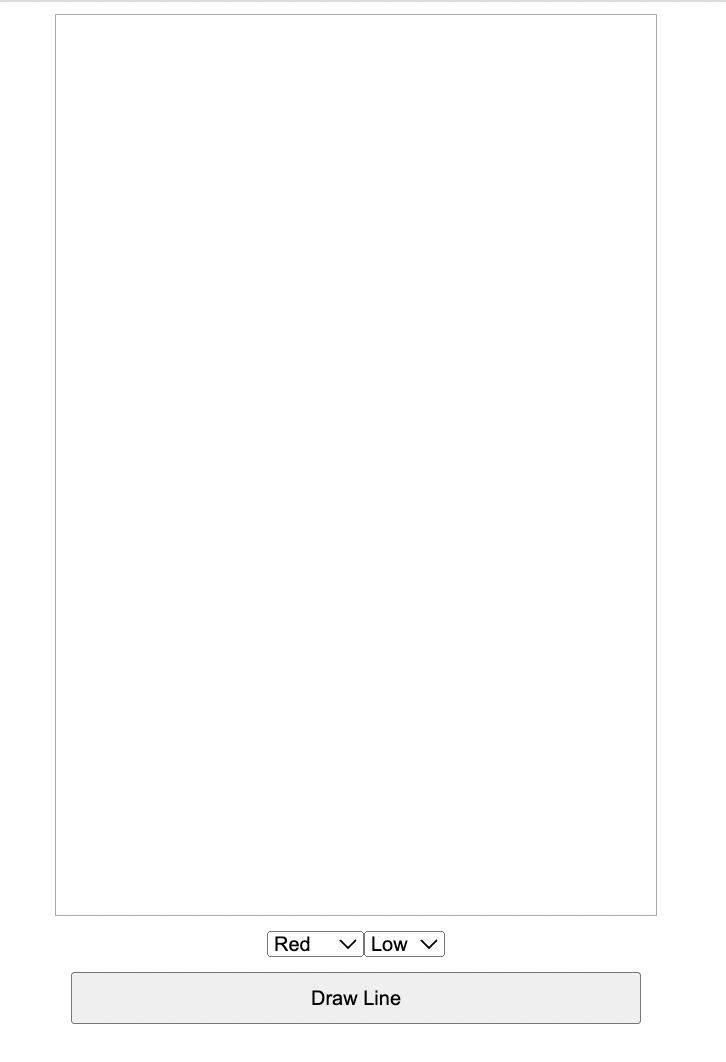
\includegraphics[width=0.3\textwidth]{ug/pic/racing_lines.png}.
    \caption{Web interface of racing\_lines.links}
    \label{fig:racing_lines}
\end{figure} 

As illustrated in Figure \ref{fig:racing_lines}, the rectangular region at the top of the canvas is where the fibers are displayed. The dropdown menu offers 6 colors and 2 priority levels, namely, ``Low" and ``High". Users can then select their desired line color and priority level for the fiber from the dropdown menu. Once they have made their selections, they can render the chosen fiber as a horizontal line on the canvas by clicking the ``Draw Line" button.

\begin{figure}[htbp]
\centering
\begin{minipage}[t]{0.48\textwidth}
\centering
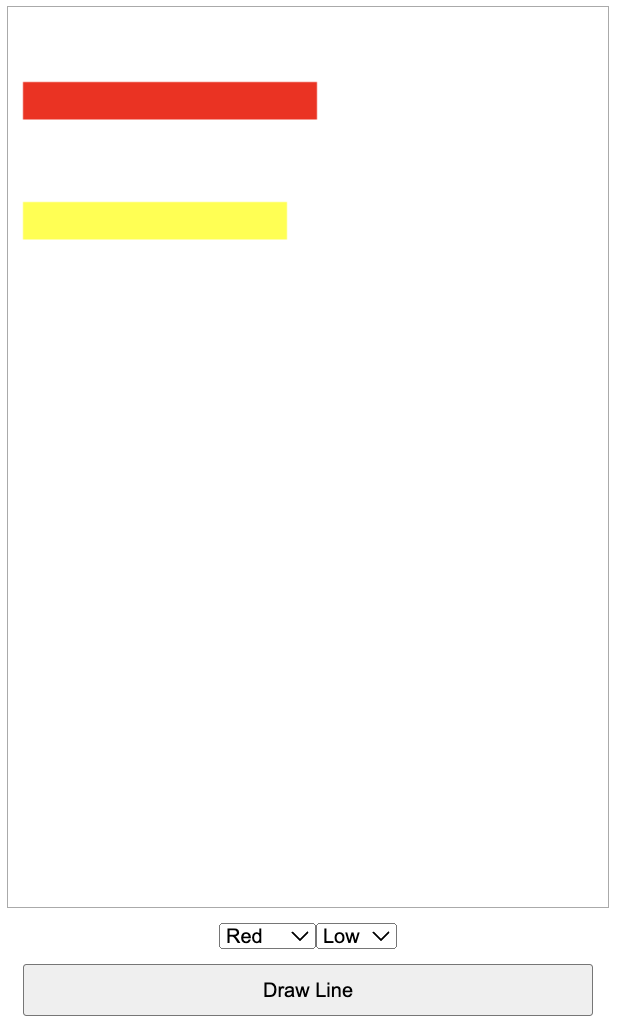
\includegraphics[width=4cm]{ug/pic/racing_lines_before.png}
\caption{Rendering process of the High-priority fibers}
\label{fig:racing_lines_before}
\end{minipage}
\begin{minipage}[t]{0.48\textwidth}
\centering
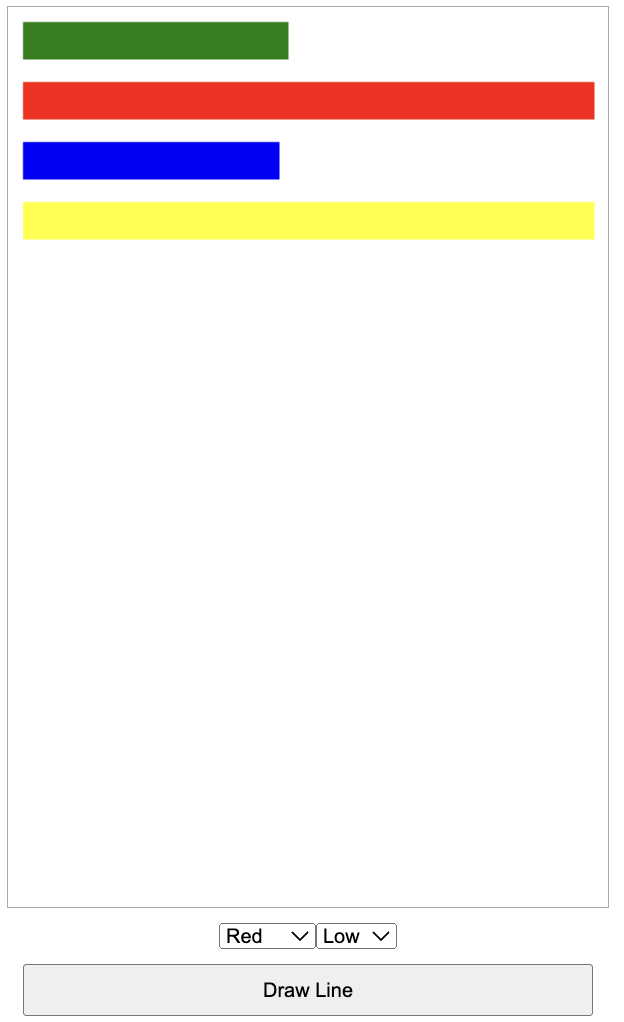
\includegraphics[width=4cm]{ug/pic/racing_lines_after.png}
\caption{Rendering process of the Low-priority fibers}
\label{fig:racing_lines_after}
\end{minipage}
\end{figure}

In Figure \ref{fig:racing_lines_before} and \ref{fig:racing_lines_after}, the process of creating four fibers is shown. First, the green fiber with low priority is created, followed by the red fiber with high priority, then the blue fiber with low priority, and finally the yellow fiber with high priority. It can be observed that, although the green fiber is the first to be created, it is interrupted during its rendering process by the red fiber because the red fiber has a higher priority. Similarly, the rendering process of the blue fiber is also blocked due to the fact that it has lower priority than the red fiber. On the other hand, since the yellow fiber has the same priority as the red fiber, both fibers will be rendered alternatively. The green and blue fibers can only resume their rendering process after the red and yellow fibers finish rendering and give control back to the lower-priority fibers. Then, they will resume their rendering process and render alternatively until they complete their rendering process.

The \texttt{racing\_lines.links} program is implemented using effect handlers to create a fiber scheduler. The scheduler uses two operations, Fork and Yield, to create fiber instances and control their interruption and resumption. The fibers are maintained in a scheduler queue and will be popped out from the queue once they finish rendering.

\chapter{Design and Implementation}
\label{chap:design_implementation}

The work presented in Section \ref{section:racing_lines} has provided a solid foundation for this project. In this section, I will provide a comprehensive explanation of the design and implementation details of the applications and schedulers that aim to enhance the user experience and simplify the deployment of different effect handlers for the same effectful operations.

\section{Overview}
\label{section:design_overview}

The user interface design of the application has been revised to enhance the user experience. To simplify the process of creating fibers with different priorities, the color and priorities dropdown menu has been merged into one.  Instead of allowing users to select from six different colors, each priority level can be assigned a specific color, such as red for Low priority and green for High priority. This change allows users to create fibers as lines on the canvas more efficiently with just one click instead of three. Additionally, each priority level has been assigned a specific color, making it easier for users to identify the state of the fibers. These improvements enable users to focus on the main task of the application, which is to create fibers and observe their behaviors when encountering fibers with different priorities that may preempt the control flow. A detailed description of the user interface implementation will be provided in Section \ref{section:user_interface}.

To enhance the user experience of the application and show the strength of Links in concurrent programming, the user interface design can be further improved by providing more priority levels for fibers. In addition to Low and High, a Medium Fiber can be introduced, represented by the color blue. This new priority level would allow the fiber to preempt the control of a Low Fiber but would need to give up the control to High Fibers. This expansion of priority levels offers more possibilities for visualizing fiber behavior and allows users to explore a wider range of scenarios. More importantly, by introducing three priority levels, Links can demonstrate its superiority in concurrent programming compared to other modern front-end frameworks. For instance, React's Concurrent Mode \cite{react_concurrent} only supports two levels of priority due to the single-threaded nature of JavaScript. The specific implementation of the user interface with three priority levels will be discussed in Section \ref{section:queue}.

In order to expand the capabilities of Links in concurrent programming, it is necessary to increase the level of control over the fiber scheduler. The goal is to have better control over the fibers, such as the ability to retrieve and modify the priority level of a fiber. Currently, the effect handler only provides the functionality to create a new fiber and yield control from one fiber to another. To achieve this objective, two new operations, namely \texttt{GetPrio} and \texttt{SetPrio}, can be defined and added to the effect handler. These new functionalities will enhance the versatility of the application and provide developers with more options to manipulate the fibers. Further details regarding the implementation of \texttt{SetPrio} and \texttt{GetPrio} will be presented in Section \ref{section:edit_prio}, highlighting the potential benefits of the Links programming language in concurrent programming.

Lastly, in the current implementation, all functionalities of the application, including the HTML, CSS code for the web interface, the JavaScript FFI for handling the drawing function on the canvas, Links code for maintaining the scheduler queue, as well as the fiber scheduler written in effect handlers, are all contained in one file. It would be more desirable to separate these functionalities into different modules, which aligns with standard software engineering coding practices. This would not only make the code more organized and easier to maintain, but also improve its reusability and extensibility in the long run. The details of how to modularize the code will be discussed in Section \ref{section:modularization}.

\section{Three Priority Level}
\label{section:queue}

The addition of one more priority level is being implemented first as it is the core functionality of the program. Before discussing the technical details of how to add the additional priority level, a brief overview of how fibers are created, stored, and scheduled by the schedulers is necessary. Each fiber has two states, \texttt{prio} and \texttt{f}, representing its priority level and the function that will be executed when the fiber is scheduled. In the two priority levels setting, fibers are stored in separate priority queues for Low and High Priority. These two priority queues are combined into one data structure called \texttt{PrioQueue} for better management. During the enqueue stage, fibers are enqueued to their respective priority queues based on their \texttt{prio} value. During the dequeue stage, fibers with High Priority are dequeued first, followed by fibers with Low Priority only if the High Priority Queue is empty. This ensures that High Priority fibers can always run before Low Priority fibers when performing the \texttt{Yield} operation. A diagram illustrating how the \texttt{PrioQueue} work is presented in Figure \ref{fig:queue}.

\begin{figure}[htbp]
    \centering
    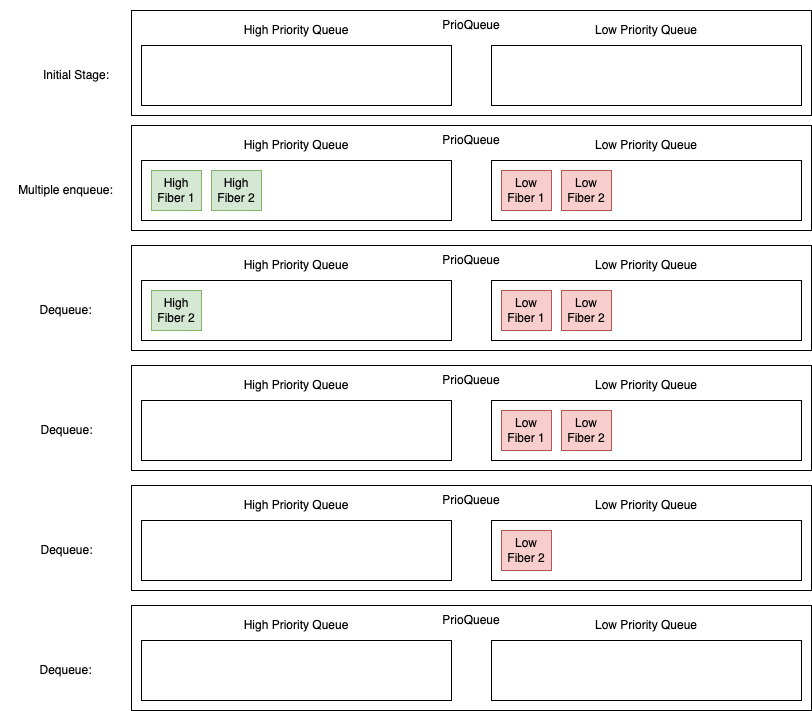
\includegraphics[width=0.75\textwidth]{ug/pic/queue.png}.
    \caption{PrioQueue behavior for fibers with different priorities}
    \label{fig:queue}
\end{figure}

The fiber scheduler, which is responsible for managing all the fibers, is implemented using effect handlers and interprets two operations: \texttt{Fork} and \texttt{Yield}.  While Section \ref{section:schedulers} provides a detailed explanation of the fiber scheduler, this section focuses on priority processing. In the \texttt{Yield} operation definition, its implementation processes the rendering function on the canvas and yields control to other fibers depending on the scheduling scheme. In the \texttt{Fork} operation definition, it determines whether the newly forked fiber should interrupt the current running fiber or be stored in the \texttt{PrioQueue} for later use using a switch statement. To add another priority level, it is necessary to modify the \texttt{PrioQueue} data structure to accommodate the new priority level, adjust the enqueue and dequeue logic accordingly, and change the implementation of the \texttt{Fork} and \texttt{Yield} operations.

The modifications made include defining a new queue for fibers with medium priority to the \texttt{PrioQueue} data structure, as well as modifying the \texttt{priorityEnqueue} and \texttt{priorityDequeue} functions to accommodate this change. The structure of the new \texttt{PrioQueue} has been illustrated in Figure \ref{fig:new_queue}.

\begin{figure}[htbp]
    \centering
    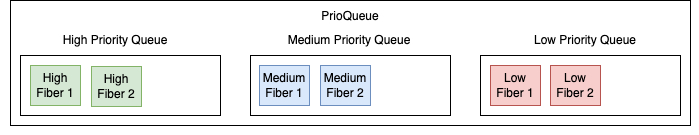
\includegraphics[width=0.75\textwidth]{ug/pic/new_queue.jpg}.
    \caption{new PrioQueue structure}
    \label{fig:new_queue}
\end{figure}

Furthermore, in order to integrate the new \texttt{PrioQueue} structure to the fiber scheduler, the \texttt{Fork} operation definition was also modified to incorporate the relationship between low, medium, and high priority fibers, allowing newly created fibers to preempt lower-priority fibers and enqueued into the \texttt{PrioQueue} if the current running fiber has a higher priority. The \texttt{Yield} operation was also updated to include the rendering process for fibers with medium priority. A more detailed explanation of the fiber schedulers can be found in Section \ref{section:schedulers}.

\section{User Interface Implementation}
\label{section:user_interface}

Now that the implementation of the three priority levels is complete, the focus can now shift towards improving the user interface of the application. As shown in Figure \ref{fig:racing_lines}, the current process of creating a new fiber requires users to interact with two separate dropdown menus to select the color and priority of the fiber, followed by clicking the "Draw Line" button, which involves three clicks. This process can be further simplified by reducing the number of clicks required to create a fiber to one, providing users with greater convenience and more straightforward control over the creation of fibers.

In the current implementation of the application, the \texttt{buttonPressed} function is linked to the \texttt{button} tag in the code using l-event attributes. This function will be executed when a click event on the button is detected. It retrieves the values for priority and color using the \texttt{getValueFromSelection} function, and then it uses switch statement to determine the priority level of the fiber, with the appropriate action taken based on the priority level. The code for the \texttt{buttonPressed} function is shown below:

\begin{verbatim}
fun buttonPressed(){
    var prio = getValueFromSelection("prio");
    var f = setUpLineDrawing(getValueFromSelection("line-color"));
    switch(prio){
        case "High" -> sysEnqueue(makeFiber(High, f))
        case "Medium" -> sysEnqueue(makeFiber(Medium, f))
        case "Low" -> sysEnqueue(makeFiber(Low, f))
        case _ -> ()
    }
}
\end{verbatim}

Based on the design choice discussed in Section \ref{section:design_overview}, the two dropdown menus and the "Draw Line" button functionalities can be simplified into one single button for users. This new button should enable users to create a fiber with a fixed color and priority level. In order to achieve this, three buttons are needed, with each button responsible for creating fibers of a specific color and priority level. The implementation can be accomplished by replacing the HTML code for the dropdown menus and button with the new code for the three buttons. Additionally, since the dropdown menus are no longer necessary, the buttonPressed function can be updated to hardcode the values for priority and color. As a result, the existing code can be replaced from:
\begin{verbatim}
<div class="selection margin-10 center">
    <select id="line-color">
        <option value="red">Red</option>
        <option value="green">Green</option>
        <option value="blue">Blue</option>
        <option value="yellow">Yellow</option>
        <option value="#801638">Berry </option>
        <option value="#027878">Teal</option>
    </select>
    <select id="prio">
        <option value="Low">Low</option>
        <option value="Medium">Medium</option>
        <option value="High">High</option>
    </select>
</div>
<button class="block button center" l:onclick="{buttonPressed()}">
    Draw Line
</button>
\end{verbatim}

to the new code as shown below:

Note: Should I give the better name for the button
\begin{verbatim}
<div class="selection margin-10 center">
    <button 
        class="block button center" 
        l:onclick="{buttonPressed("Low", "red")}">
        Draw Low Line
    </button>
    <button 
        class="block button center" 
        l:onclick="{buttonPressed("Medium", "blue")}">
        Draw Medium Line
    </button>
    <button 
        class="block button center" 
        l:onclick="{buttonPressed("High", "green")}">
        Draw High Line
    </button>
</div>
\end{verbatim}

The proposed modifications to the user interface simplify the process of creating fibers and improve user experience by making the interface more intuitive and user-friendly. Additionally, these changes result in cleaner and more maintainable code.  It is important to note that the function signature of \texttt{buttonPressed} is modified to receive hardcoded color and priority values as arguments, which leads to a revised implementation for \texttt{buttonPressed}. The new function implementation is shown below:
\begin{verbatim}
fun buttonPressed(prio, color){
    var f = setUpLineDrawing(color);
    switch(prio){
        case "High" -> sysEnqueue(makeFiber(High, f))
        case "Medium" -> sysEnqueue(makeFiber(Medium, f))
        case "Low" -> sysEnqueue(makeFiber(Low, f))
        case _ -> ()
    }
}    
\end{verbatim}

Finally, the user interface before and after the modifications are displayed in Figure \ref{fig:ui_before} and Figure \ref{fig:ui_after}, respectively.

\begin{figure}[htbp]
\centering
\begin{minipage}[t]{0.48\textwidth}
\centering
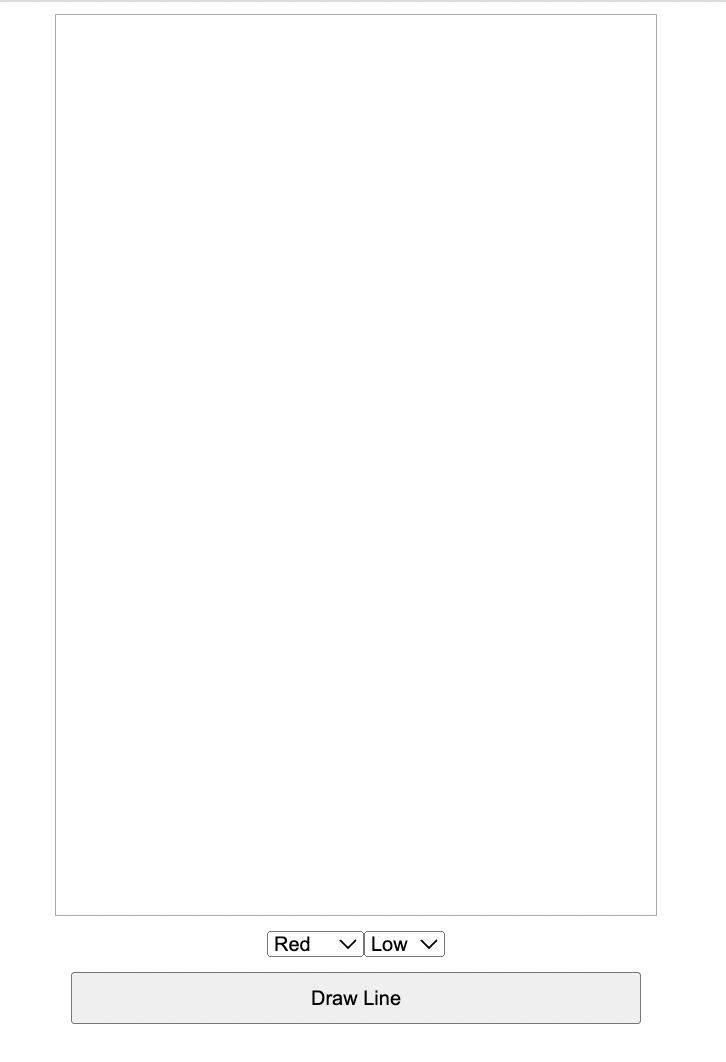
\includegraphics[width=4cm]{ug/pic/racing_lines.png}
\caption{Before modification}
\label{fig:ui_before}
\end{minipage}
\begin{minipage}[t]{0.48\textwidth}
\centering
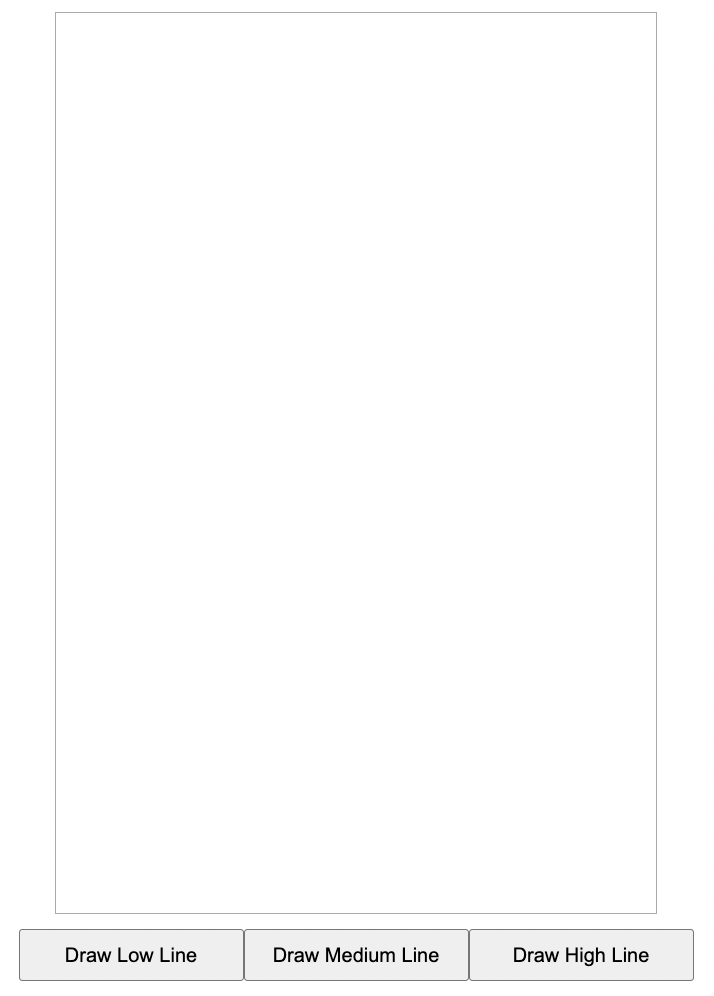
\includegraphics[width=4cm]{ug/pic/ui_after.png}
\caption{After modification}
\label{fig:ui_after}
\end{minipage}
\end{figure}

\section{Editing Priority of the Fiber}
\label{section:edit_prio}

As I described in Section \ref{section:handler}, defining an operation inside the effect handlers requires providing both of its definition and implementation. Defining the \texttt{GetPrio} operation is straightforward since the state of the fiber can be accessed by having an additional parameter in the handle function. Therefore, every time this operation is captured by the handlers, we can simply resume the current rendering process and return the current priority level back to the client.

The \texttt{SetPrio} operation is more challenging to implement than \texttt{GetPrio} since it requires updating both the priority level in the fiber's state and its position in the correct Priority Queue inside the \texttt{PrioQueue} data structure shown in Figure \ref{fig:new_queue}. To implement \texttt{SetPrio}, a parameter \texttt{p} for priority level is defined in the operation definition, and a helper function called \texttt{newPrioToFiber} is defined. This function takes \texttt{p} as an argument, creates a new fiber with the same information as the original fiber but with the priority level changed to the selected level, and enqueues this new fiber into the appropriate Priority Queue in \texttt{PrioQueue}. The scheduler will then yield control to the next fiber according to its scheduling scheme.

The implementation code for \texttt{GetPrio} and \texttt{SetPrio} operations is presented below. The variable \texttt{state} holds the current state of the fiber's scheduler, including its priority level and the \texttt{PrioQueue} data structure. This state is passed to the handler function, so that the operations can be executed within the context of the current fiber's state. As the fiber interacts with the operations defined in the program, the \texttt{state} parameter is updated throughout the execution of the fiber.

\begin{verbatim}
handle(fiber.f()) ( state <- (
                        prio=fiber.prio, 
                        runQ=runQ
                    )){
    case x -> runNext(poll(state.runQ))
    case <GetPrio => resume> -> resume(state.prio, state)
    case <SetPrio(p) => resume> -> 
            var q = fiberEnqueue(newPrioToFiber(resume, p), state.runQ);
            runNext(poll(q))
    case <Fork(f) => resume> -> ...
    case <Yield => resume> -> ...
}
\end{verbatim}

\section{Modularization}
\label{section:modularization}

The next step is to improve the overall quality of the program and make it more maintainable, readable and modular. To achieve this, the application can be first broken down into separate functionalities as follows:
\begin{itemize}
  \item HTML and CSS code for the web user interface
  \item Links code for the fibers and fiber schedulers
  \item Links code for the scheduler queues, including its enqueue and dequeue functionalities
  \item Links code for the user interaction
  \item Links code for handling drawing functionalities
  \item JavaScript FFI for accessing the actual canvas rendering functionalities
\end{itemize}

The process of separation has been divided into two sections. Section \ref{soc} focuses on the modularization process, which separates each individual functionality into separate modules. On the other hand, Section \ref{eei} focuses on the separation process specifically in the context of effect handlers.

\subsection{Seperation of Concerns}
\label{soc}
The relationships and dependencies between the program's functionalities must be analyzed to begin the modularization process. For instance, the scheduler queue and fibers are used inside the scheduler. Furthermore, the main application consists of two JavaScript FFIs, one to invoke JavaScript functions (\texttt{canvas.js}) to render the lines on the canvas, and the other is to hold a similar scheduler queue in the JavaScript runtime (\texttt{runtime.js}), which will be discussed further in Section \ref{runtime}. Additionally, the main application also contains Links code to retrieve and update the coordinates on the canvas to facilitate line rendering. 

To enhance the maintainability and extendibility of the codebase, it is suggested to separate the functionalities into separate files. The main application should only contain user interaction code while the other functionalities should be split into separate files. This design decision will help in managing the codebase effectively and improving overall code quality.

After the separation process, the file \texttt{racingLines.links} will have dependencies on the files \texttt{racingLines.css} and \texttt{lineDrawer.links}, while \texttt{scheduler.links} will depend on \texttt{queue.links}. Furthermore, the two JavaScript files, namely \texttt{canvas.js} and \texttt{runtime.js}, are being used for the JavaScript FFI, which will be utilized in both \texttt{scheduler.links} and \texttt{racingLines.links}. The file structure of the application before and after the separation of concerns is shown in the left and right panels, respectively.


\begin{multicols}{2}
\dirtree{%
.1 /.
.2 /js.
.3 runtime.js.
.3 canvas.js.
.2 racing\_lines.links.
}
\columnbreak
\dirtree{%
.1 /.
.2 /js.
.3 runtime.js.
.3 canvas.js.
.2 /css.
.3 racingLines.css.
.2 scheduler.links.
.2 LineDrawer.links.
.2 queue.links.
.2 racingLines.links.
}
\end{multicols}

The separation of the code into individual functionalities not only allows developers to work on specific functionalities without conflicts, but also makes it easier to identify and resolve bugs, since issues can be isolated to specific modules, thereby improving the stability and reliability of the application.

\subsection{Extract Effect Interface}
\label{eei}
Note: I'm not sure if I express effect interface correctly

To achieve the primary objective of providing a more convenient approach for the application to use different effect handlers on the same effectful operations, it is essential to extract the effect interface into its own module.  The effect interface represents a function or set of functions that execute an effectful operation. This separation ensures the application to execute on the same operation sets, regardless of the effect handlers (schedulers) we integrate. This allows to integrate various implementations of scheduling schemes on the same operations.

The application includes four effect interfaces, each responsible for a specific set of operations such as creating a new fiber, yielding control to another fiber, get and set the priority level of the fiber. These four effect interfaces will be extracted into a new file called \texttt{fiberInterface.links}. Additionally, some helper functions such as \texttt{makeFiber} will also be included in this file, as it is related to the functionality of fiber creation. The details of this decision will be further discussed in Section \ref{runtime}.

After this modification, \texttt{racingLines.links} and \texttt{scheduler.links} modules will incorporate the functionalities and types offered by the \texttt{fiberInterface.links} module to create and manipulate the fibers. The updated file structure is as follows:

\dirtree{%
.1 /.
.2 /js.
.3 runtime.js.
.3 canvas.js.
.2 /css.
.3 racingLines.css.
.2 scheduler.links.
.2 LineDrawer.links.
.2 queue.links.
.2 fiberInterface.links.
.2 racingLines.links.
}

\subsection{runtime.js}
\label{runtime}
Note: Should I discuss about the challenge here or in evaluation?

As this project mainly focuses on Links, minimizing or eliminating the dependency on JavaScript FFI has been attempted. Despite this effort, the use of \texttt{canvas.js} could not be avoided due to the lack of support for the Canvas API in Links, making it dependent on JavaScript. On the other hand, a significant amount of  time and effort was invested in attempting to remove \texttt{runtime.js} from the application. This file has functionalities such as delaying the execution time for line rendering to improve inspection and managing fibers, which can, in theory, be replaced by the Links code.

The main purpose of the \texttt{runtime.js} file is to manage fibers in the JavaScript runtime by providing functionalities such as an external scheduler queue that temporarily stores newly created fibers triggered by button-click events. This scheduler queue includes its own enqueue and dequeue functions. When a button is clicked, the application creates a new fiber using the \texttt{makeFiber} function. Instead of performing a \texttt{Fork} operation, the enqueue function of the external scheduler queue is called, and the new fiber is added to this queue. Then, when the scheduler decides to yield control to other fibers, it first calls the dequeue function of the external scheduler queue to load the fibers from the external queue into the actual \texttt{PrioQueue}. The scheduler then selects the next appropriate fiber in the \texttt{PrioQueue} to run according to its scheduling scheme. The entire process of fiber creation and yielding has been presented in Figure \ref{fig:runtimequeue}.

\begin{figure}[htbp]
    \centering
    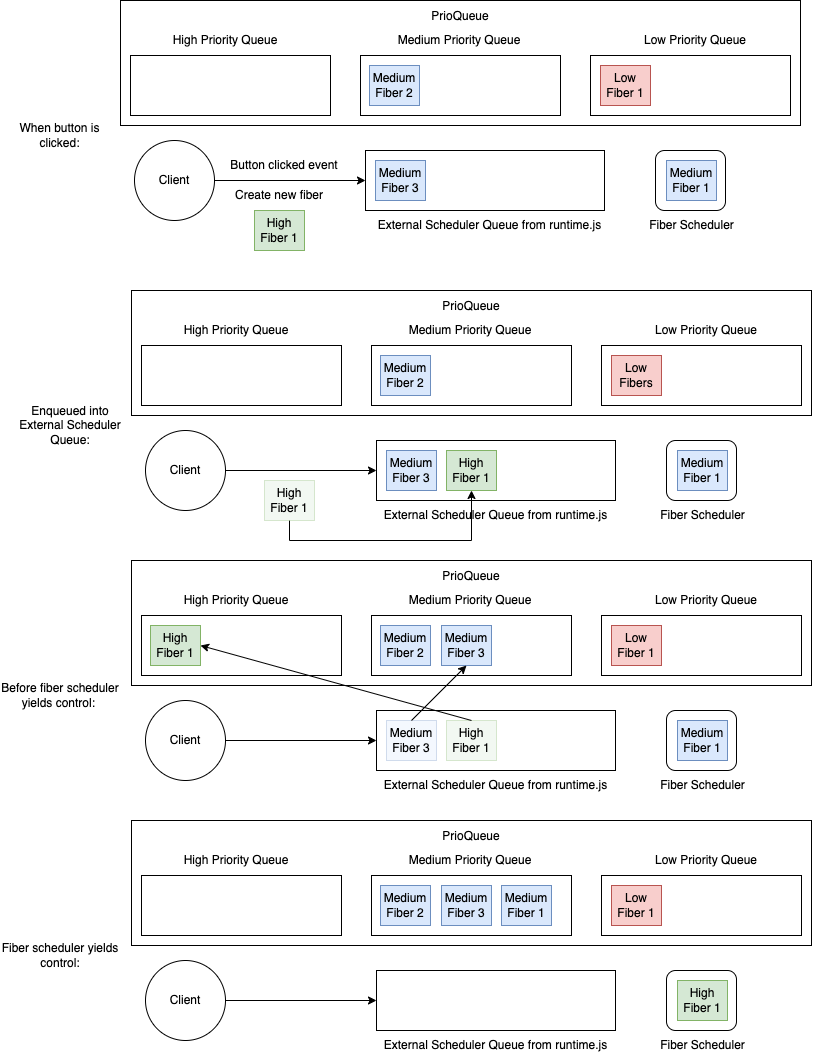
\includegraphics[width=1\textwidth]{ug/pic/runtimejs.png}.
    \caption{How external scheduler queue interacts with PrioQueue}
    \label{fig:runtimequeue}
\end{figure}

The implementation of the program has resulted in the \texttt{Fork} operation being bypassed altogether. This goes against the principle of using effect handlers, as every action affecting the fiber should be carried out using operations. The use of \texttt{runtime.js} as JavaScript FFI for fiber management is a workaround that negates the use of operations. Therefore, there is a requirement to address the interpretation of the \texttt{Fork} operation and eliminate the use of the external scheduler queue in order to comply with the principles of using effect handlers.

One potential solution to address the bypassing of the \texttt{Fork} operation is to replace all enqueue functions with \texttt{Fork} operations. However, this approach may not work as expected since the event listener of the button is not handled as part of the computational context managed by the scheduler. As a result, this approach may lead to compile-time errors. Thus, a more nuanced solution is needed, which involves handling the event listener within the context of the scheduler to properly execute the \texttt{Fork} operation.

An alternative approach to solving the problem of bypassing the \texttt{Fork} operation is to use the actor model, which was introduced in Section \ref{section:bg_concurrent_programming} and is built into Links. The actor model replaces the event listener and uses a message-passing mechanism where each button clicks event dispatches a message to a receiver that executes the corresponding functionality based on the message. A comparison between the implementation of the actor model-based receiver and the event listener has been presented below.
\begin{verbatim}
// Agent model-based
fun receiver(){
    Scheduler.yield();
    receive {
        case CreateLowLine -> buttonPressed("Low", "red")
        case CreateMediumLine -> buttonPressed("Medium", "blue")
        case CreateHighLine -> buttonPressed("High", "green")
    };
    receiver()
}

fun main_page(_){

    var pId = spawnClient{
        Scheduler.schedule(Scheduler.makeFiber(High, receiver))
    };
      ...
    <button l:onclick="{pId ! CreateHighLine}">
        Draw High Line
    </button>
      ...
}
\end{verbatim}  
\begin{verbatim}
// Event listener based
fun main_page(){

    var pId = spawnClient{
        schedule(FiberInterface.makeFiber(High, start))
    };

    ...
    <button l:onclick="{buttonPressed("High", "green")}">
        Draw High Line
    </button>
    ...        
}
\end{verbatim}

By merging the three event listeners into one \texttt{receiver} function, it provides the advantage of enabling the scheduler to handle this function, which enables the possibility to perform the \texttt{Fork} operation. This approach eliminates the need to use \texttt{runtime.js}.

The approach described above, although promising, resulted in unexpected issues due to a false assumption made in the initial design. It was assumed that the \texttt{receiver} function listens for the message asynchronously, but in reality, the synchronous listening process of the \texttt{receiver} function blocks the rendering process, which in turn, blocks the entire scheduler when it is waiting for the message. As a result, if a button is clicked, the newly created fiber is only able to draw a portion of the line before yielding to the next fiber. Then, after the next fiber resumes its computation, the entire execution is blocked at the \texttt{receive} block until the user clicks the ``Draw Line" button again. This behavior makes the implementation unsuitable for the intended purpose.

\begin{verbatim}
fun receiver(){
    Scheduler.yield();
    /*
    The following code block leads to execution blocking upon fiber
    resumption until a new message is passed to the receiver function:
    */
    receive { 
        case CreateLowLine -> buttonPressed("Low", "red")
        case CreateMediumLine -> buttonPressed("Medium", "blue")
        case CreateHighLine -> buttonPressed("High", "green")
    };
    receiver()
}
\end{verbatim}

Although frustrating, This issue exposes the current limitations of wrapping a single effect handler around all event handlers in Links. In addition, there is a mismatch between effect handlers and actors, making it difficult to integrate the \texttt{receiver} function into the cooperative concurrency context of effect handlers. Therefore, currently, the only option is to use shared state and implement communication between event listeners and effect handlers through \texttt{runtime.js} using JavaScript FFI.

\section{Schedulers}
\label{section:schedulers}

The heart of this project is the scheduler, which works in conjunction with the \texttt{PrioQueue}. To achieve our objective stated in Section \ref{section:objectives}, it is necessary to implement multiple schedulers with different fiber scheduling schemes. This serves as the foundation for the later implementation in Section \ref{section:merge} which focuses on enabling the easy switching of schedulers within the application. The objective is to make the application run smoothly while also making it easy for developers to switch between different effect handlers with minimal code changes. Ultimately, the aim is to simplify the process enough that only a few lines of code are necessary to switch between different effect handlers.

Before delving into the specific design and implementation of each different fiber scheduler, it is important to provide an overview of how a fiber scheduler operates in general. When a fiber is created, the scheduler determines whether it should be executed by comparing its priority level with that of the currently running fiber. The unselected fiber will be enqueued into the \texttt{PrioQueue}, while the selected fiber will execute by rendering a slice of lines on the canvas until the scheduler decides to yield control. If the executing fiber is not finished yet when the scheduler yields control, it is re-enqueued to the \texttt{PrioQueue} before yielding. However, if it finishes executing, it simply returns. The scheduler yields control by selecting the next fiber dequeued from the \texttt{PrioQueue} using the specified scheduling scheme. This process continues until the \texttt{PrioQueue} is empty. The flowchart of the scheduler operation is illustrated in Figure \ref{fig:scheduler}. With this general understanding in mind, we can now proceed to explore the specific design and implementation of each different fiber scheduler.

\begin{figure}[htbp]
    \centering
    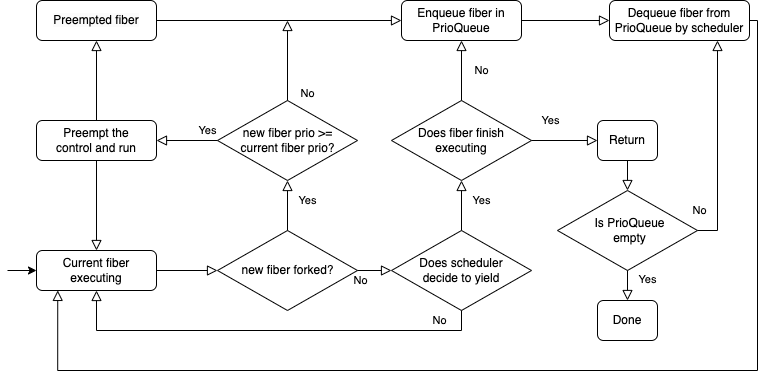
\includegraphics[width=.7\textwidth]{ug/pic/scheduler.png}.
    \caption{Flowchart of how the fiber scheduler operates}
    \label{fig:scheduler}
\end{figure}

The following sections present the design for the three schedulers that we developed: time-based, steps-based, and probability-based schedulers. Each section provides an overview of how the scheduler operates, along with a diagram to aid in understanding. We also present the actual implementation of the scheduler and the modifications made to the \texttt{PrioQueue} and effect handlers to achieve it.

\subsection{Time-based Scheduler}

The time-based scheduler is designed to allocate different execution times to fibers based on their priority levels. When yielded by the scheduler, high-priority fibers are allocated 400ms, medium-priority fibers are allocated 200ms, and low-priority fibers are allocated 100ms for execution. This approach enables higher-priority fibers to execute their operations for a longer period of time before yielding control, enabling them to complete their execution more quickly than lower-priority fibers.

The structure of the \texttt{PrioQueue} and the enqueue and dequeue functions remain the same as described in Section \ref{section:queue}, where the fiber with the highest priority is dequeued first, and lower-priority fibers are dequeued only when the queues for higher-priority fibers are empty. The precise process of this scheduling scheme and the \texttt{PrioQueue} structure is illustrated in Figure \ref{fig:scheduler_time} below.

\begin{figure}[htbp]
    \centering
    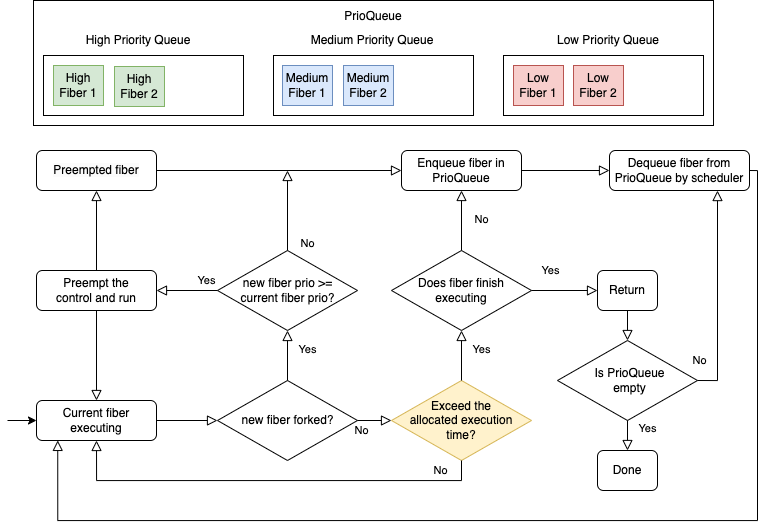
\includegraphics[width=.7\textwidth]{ug/pic/scheduler_time.png}.
    \caption{Time-based Scheduler}
    \label{fig:scheduler_time}
\end{figure}

As can be observed, the modifications required for implementing the time-based scheduler are narrowed down to the Yield operation and the state structure attached to the handler, as the \texttt{PrioQueue} remains unchanged. Specifically, a new state field named \texttt{startTime}, which represents the start time of the fiber's execution in milliseconds, needs to be added. Upon yielding control, the \texttt{startTime} of the next running fiber is updated. Then, execution times are assigned to fibers according to their priority levels, and we must check if the fiber has used up its allocated execution time. If not, the fiber's execution is resumed; otherwise, control is yielded to the next fiber. The main code implementing these modifications is provided below.

\begin{verbatim}
handle(fiber.f()) ( state <- (
                        prio=fiber.prio, 
                        runQ=runQ, 
                        startTime=clientTimeMilliseconds()) 
                    ){
    ...
    case <Yield => resume> ->
        var currentTime = clientTimeMilliseconds();
        var buffer = switch(state.prio){
            case High -> 400
            case Medium -> 200
            case Low -> 100
        };
        if (currentTime - state.startTime <= buffer) {
            resume((), state)
        } else{
            var q = fiberEnqueue(
                        resumptionToFiber(resume, state.prio), 
                        state.runQ
                    );
            runNext(poll(q))
        }
}
\end{verbatim}

\subsection{Steps-based Scheduler}

\subsection{Probability-based Scheduler}

\section{Switch Schedulers}
\label{section:merge}

The next step after defining and implementing the three schedulers is to integrate them into the application and allow users to switch between them. To achieve this, the schedulers need to be parameterized as variables that can be passed as arguments to the application. Our solution is to define each scheduler as a subroute inside the main function and pass it as an argument to the page generation function. To facilitate this, three clickable links are added to the user interface, allowing users to switch between schedulers by clicking the appropriate link. Upon clicking a link, the browser refreshes and navigates to the designated subroute for the selected scheduler. The scheduler is then passed to the page generation function and used to initialize the schedulers. The modified code to enable this functionality has been provided.
\begin{verbatim}
- fun main_page(_){
+ fun main_page(schedule){
    - var pId = spawnClient{Scheduler.schedule(makeFiber(High, start))};
    + var pId = spawnClient{schedule(FiberInterface.makeFiber(High, start))};

    page
    <HTML>
    ...
    <body>
        + <a href="/scheduler1.links">Scheduler 1</a>
        + <a href="/scheduler2.links">Scheduler 2</a>
        + <a href="/scheduler3.links">Scheduler 3</a>
    </body>
    </html>
}

fun main() {
    ...
    - addRoute("/", main_page);
    + addRoute("/", fun(_) {main_page(Scheduler.schedule)});
    + addRoute("/scheduler1.links", fun(_) {main_page(Scheduler1.schedule)});
    + addRoute("/scheduler2.links", fun(_) {main_page(Scheduler2.schedule)});
    + addRoute("/scheduler3.links", fun(_) {main_page(Scheduler3.schedule)});
    servePages()
}
main()
\end{verbatim}

This modification greatly simplifies the process of adding or removing schedulers from the application. The developer only needs to add a subroute in the main function and a hyperlink on the UI that links to this subroute, which only requires two lines of code. Users can then switch between schedulers during runtime by clicking the hyperlink. This approach achieves our objective of making it easy for developers to switch and integrate different effect handlers with minimal changes to the code.

\section{Applications}

The objective now is to validate the general applicability of our scheduler switching approach by building three different applications that exhibit distinct rendering behaviors. This is necessary to ensure that our scheduler switching approach is not limited to a specific type of application and can work effectively across various contexts. Once the applications are developed, we will evaluate and test them in detail in Chapter \ref{chap:evaluation} to demonstrate the ease and robustness of incorporating different schedulers and ensuring the correct functioning of the applications.

In general, the application works as follows: when the user clicks a button, the corresponding event listener triggers the \texttt{buttonPressed} function. This function creates the fiber based on the priority level, and the fiber is enqueued into the external scheduler queue in \texttt{runtime.js} through JavaScript FFI. The fiber is later dequeued and stored in the actual \texttt{PrioQueue} when the fiber scheduler yields control. The fiber has two properties: its priority level and a drawing function responsible for rendering lines on the canvas. During the fiber's execution, the rendering function is invoked, which draws the line slice by slice by calling the \texttt{drawCustomUnit} function in \texttt{canvas.js} through JavaScript FFI. The scheduler tries to yield control every time a slice of line is rendered. When the rendering process is complete, the function's execution finishes, and the fiber is returned.

\subsection{Application 1}
This is a general and intuitive rendering behavior, where each fiber starts from the left and proceeds towards the right of the canvas. Once the line reaches the right edge of the canvas, it is considered finished and the fiber returns from the effect handlers. A visual representation of this behavior is provided in Figure \ref{fig:app1}. As illustrated, the low-priority fiber is created first and starts rendering. However, its execution is interrupted when the higher-priority fiber is created and takes control of the execution. The higher-priority fiber then renders until completion before the lower-priority fiber resumes rendering until it is also finished.

\begin{figure}[htbp]
    \centering
    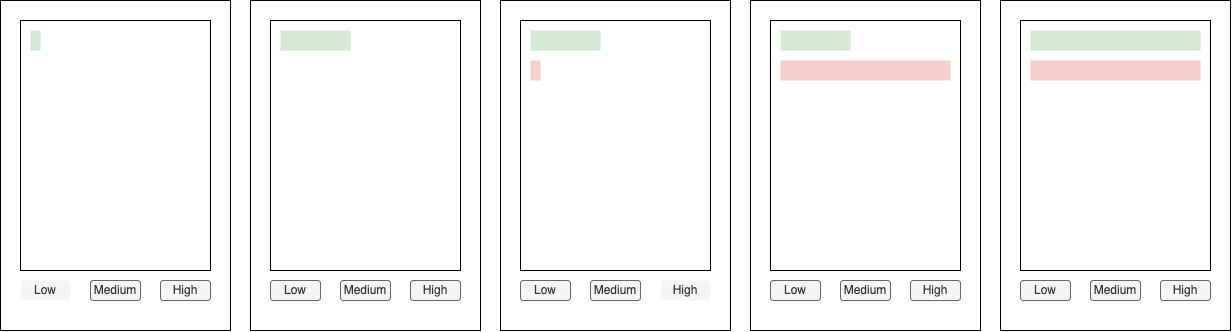
\includegraphics[width=.8\textwidth]{ug/pic/app1.png}.
    \caption{Rendering behavior of application 1}
    \label{fig:app1}
\end{figure}

The implementation of the rendering function begins by obtaining the \texttt{x} and \texttt{y} coordinates for the start and end points of the line that will be drawn. Next, an inner function is defined, responsible for rendering the line slice by slice, starting from the left and moving towards the right, using the \texttt{drawCustomUnit} function. After each slice is rendered, the inner function yields control to the scheduler. Then after the resumption, the inner function delays the execution of the next slice of the line, allowing the line to be drawn progressively. The inner function repeats this process recursively until the entire line is drawn, with the \texttt{x} coordinate of the start point being updated at each iteration.

\subsection{Application 2}
\subsection{Application 3}

\chapter{Evaluation}
\label{chap:evaluation}

\section{Testing}
Notes: I was planning to go through some examples for all three applications with all three schedulers to show that they are functioning properly

\subsection{Application 1}

\subsection{Application 2}

\subsection{Application 3}

\section{Analysis of results}


Largely reduced the lines of code (from 444 to 129)

By implementing the editing priority funcitonalities in effect handlers, I also found a way to allow users to pause and resume the fibers during runtime.

Not able to create fiber through fork operation in effect handlers

No documentation of effect handlers, and several verison update during the development stage

Error messages can be very intimidating or too simple that doesn't help the debugging process

The canvas can hold maximum 15 lines, should add a scrollable functionality

\section{User Experience}

Make comparison with the original racing\_line.links example such as the ease of user interaction and switching effect handlers

\section{Challenges}
Note: This section could be deleted and move to conclusion as one paragraph

Restate Section \ref{runtime}, and highlight the impact of this problem to this project.

\section{Comparison}

Note: I'm thinking to delete this section since the original reason for making this section is because I was assuming it would be good if I can build a React version of racing line and compare it with the links version


\chapter{Conclusion and Future Works}
\label{chap:conclusions}

This project aims to enable easy switching of schedulers in web applications using Links. The main objective of this work was to create a smooth-running application that allows for effortless switching between different effect handlers with minimal code modifications. To achieve this, we added more priority options to the fibers, improved the UI design for better user interaction, modularized the program, developed multiple schedulers with different fiber scheduling schemes, and incorporated clickable links on the user interface. Additionally, we built three different applications that displayed distinct rendering behaviors to demonstrate the applicability of our approach. Lastly, we evaluated and tested the applications to demonstrate the ease and robustness of the approach, ensuring that the applications functioned correctly.

State some of the applications that could possibly make use of the fibers and schedulers (such as online gaming, video conference, chat applications)

\section{Future Works}

Implement the pause and resume of fibers

Create a version of the demo using React and compare it to the Links

Allow the user to change scheduling scheme without the need to refresh the browser

\bibliographystyle{plain}
\bibliography{mybibfile}


% You may delete everything from \appendix up to \end{document} if you don't need it.
\appendix

\chapter{Complete code for racing lines demo}

\section{racingLines.links}
\section{fiberInterface.links}
\section{lineDrawer.links}
\section{scheduler.links}


\end{document}
